\documentclass{article}
\usepackage{amsmath}
\usepackage{amssymb}
\usepackage{setspace}
\usepackage{mathrsfs}
\usepackage{ulem}
\usepackage{graphicx}
\graphicspath{ {images/} }
\begin{document}
\begin{spacing}{1.5}

You can also find the official video lecture summary on https://ocw.mit.edu/courses/mathematics/18-06sc-linear-algebra-fall-2011/ax-b-and-the-four-subspaces/the-geometry-of-linear-equations/  \qquad See the left navigation bar on this page, you will get all summaries.

\section{}
Row picture, column picture\\
Example: for\\
	$2x-y=0\\
	-x+2y=3$
	
Row picture is that draw $2x-y=0, -x+2y=3$ on coordinate and find a point satisfying the two equations. That point is the solution.

Column picture is to solve $x(2, -1)^T + y(-1, 2)^T = (0, 3)^T$. This means combine two vectors($(2, -1), (-1, 2)$) to get the final $(0,3)$ point. In addition, $x(2, -1)^T + y(-1, 2)^T$ is called {\bfseries linear combination} of columns. In column picture, for Ax=b, in view of x, every row of A makes a transform on x, resulting every new dimension value which assemble b; in view of A, combination of all its columns weighted by x, resulting b. 

So when calculate $Ax$, we can use row picture or column picture. 


\section{}
$$
\begin{bmatrix}
0 & 1 \\
1 & 0 
\end{bmatrix}
\begin{bmatrix}
a & b\\
c & d
\end{bmatrix}
=
\begin{bmatrix}
c & d \\
a & b
\end{bmatrix}
$$ 

You can get the left 0, 1, 1, 0 matrix by imagining column picture.
The result re-permutes the origin in row. If you want to re-permute it in column, write the 0, 1, 1, 0 matrix at the right-hand side of $[a, b; c, d]$.


\section{}
Part 1. Four ways to calculate $AB=C$ \\
1. The commonest way is $C_{ij} = \sum A_{ik}B_{kj}$. \\
2. But you can also focus on one column of B or C at one time. In this view, $C_{i-col} = A*B_{i-col}$. It's exactly column picture in section 1. So all columns in A are combined, weighted by one column of B at one time, resulting many columns, and these columns assemble C. \\
3. The third way is to focus on one row of A or C at one time. In this view, $A_{i-row} = A_{i-row} * B$. You can think it with imagining transpose of $C_{i-col} = A*B_{i-col}$ in the second way. \\
4. $C = \sum A_{i-col}*B_{i-row}$, the last way. I think this is the most magical way:) \\
In addition, you can also use trick of block.\\ 
\\ Part 2. \\
Inverse: $AA^{-1}=A^{-1}A=I$. \\
\\ When is a matrix A invertible?

An invertible matrix is called {\bfseries non-singular/invertible}. From the first term, you can calculate A's determinant. If it's 0, A is singular.

But there is also a magical way, if you can find a vector $x \neq 0$, satisfies $Ax=0$, A is singular. Why? If $Ax=0$, $A^{-1}Ax=x=0$, but $x \neq 0$. Why it's magical? Imagine when you can get $x \neq 0$, $Ax=0$? By column picture, it means that we can get at least one (minus) column of A by combining all of the rest columns. That's called {\bfseries linear dependence}! \\ 
\\ When A is invertible, how to get its inverse?

Concatenate A and I, write as $[A \quad I]$, and transform A to I with elementary transformation. The result is $[I \quad A^{-1}]$. This is called {\bfseries Gaussian-Jordan elimination}. Why does it work? If $A \rightarrow I$, the $\rightarrow$ must be multiplied by $A^{-1}$. So $I \rightarrow \, ?$, the ? must be $I*A^{-1}=A^{-1}$. Of course, you can use other ways to get $A^{-1}$, but I think this is the easiest way.


\section{}
$A = LU = LDU$, here L is lower triangular, D is diagonal, U is upper triangular. \\
\\ How many operations do we need to get $A_{n*n}=LU$?

We can use elementary transformation to transform A to U, the elementary matrix is $L^{-1}$. To get U, first just eliminate the first column(except for the first row), so we need about $n^2$ operations(take multiply and add as one operation and let the first row also operate on itself). Then only focus on the sub-matrix $A_{(n-1)*(n-1)}$, here we need about $(n-1)^2$ operations. The final number is $\sum_{1}^{n} i^2 = (n * (n + 1) * (2n + 1)) / 6$, simply taking it as $n^3/3$. \\
\\ How many operations do we need to get $A_{n*n}=LDU$?

We can get $A=LU^{'}$ first, and then get $U^{'}=DU$. The first step take about $n^3/3$ operations, and the second step take $n(n+1)/2$ operations. You can get this number similar to $A=LU^{'}$ step.


\section{}
Part 1. Permutation matrix

Permutation matrix is identity matrix I with reordering rows, including I.

a. There are n! permutation matrixes for $I_{n*n}$.

b. For Permutation matrix P, $P^{-1}=P^{T}$.

c. $P^{-1}=P^{T}$ is also permutation matrix.
\\\\ Part 2. Transpose

For $A=RR^T$, A is symmetric, $A=A^T$. Because $A^T=(RR^T)^T=RR^T=A$.
\\\\ Part 3. Vector space, Column space, Vector subspace

A vector space is defined as result of addition of any two vectors in this space or multiply by a scalar still lies in this space.

Column space is defined as the set of all possible linear combinations of a matrix's column vectors.

A subspace(vector subspace) is a subspace of vector space, and it also is a vector space(vector space inside vector space). For example, subspace of $R^3$ is set of $R^3$, any plane $R^2$ through origin, any line $R$ through origin. You can see that any subspace must through origin, because we can multiply a vector in the space by 0, resulting origin.

You can see that a vector space or a subspace must be $R^n$. It can't be part of $R^n$.


\section{}
Part 1.

Intersection of subspaces S and T, $S \cap T$, is also a subspace, because a subspace must be $R^n$, so the intersection is $min(S, T)$. \\
\\ Part 2. Nullspace \\
For $Ax=b$, we can get $\{x|Ax=b\}$, but is it a vector space?

When b is not 0, it's not a vector space. Because x can't be 0, and a vector space must contains 0. In detail, $\{x|Ax=b\}$ is a point, line, plate or space that doesn't go through origin. For example, you get $x(1, 0, 0)^T+y(0, 1, 0)^T+z(0, 0, 0)^T=(1, 1, 0)$ in column picture. The solution is $(1, 1, n)$, n can be any value, but the solution always can't be $(0, 0, 0)^T$.

But when b is 0, it's a vector space. Why? Suppose w, v are two solutions of $Ax=b$, $A(aw+bv)=a(Aw)+b(Av)=0$, so $aw+bv$ is also in $\{x\}$.(a,b are scalars, w,v are vectors). Specially, for A, $\{x|Ax=0\}$ is called A's {\bfseries nullspace, $N(A)$}.

\section{}
To get nullspace of A:

(i) Use {\bfseries Reduced Row-Echelon Form(RREF)} and reorder columns to get $[I, F; 0, 0]$. 

(ii) take inverse-reorder of (i) on rows of $[-F, I]^T$. Nullspace is column space of  $[-F, I]^T$. 
\\\\Explanation and example

For $Ax=0$, take three steps. Here $\{x\}$ is nullspace.
$$
\begin{bmatrix}
1 & 2 & 2 & 2 \\
2 & 4 & 6 & 8 \\ 
3 & 6 & 8 & 10 
\end{bmatrix}
\xrightarrow[change]{\{x\}\, doesn't}
\begin{bmatrix}
1 & 2 & 0 & -2 \\
0 & 0 & 1 & 2 \\ 
0 & 0 & 0 & 0
\end{bmatrix}
\xrightarrow[changes]{\{x\}}
\begin{bmatrix}
1 & 0 & 2 & -2 \\
0 & 1 & 0 & 2 \\ 
0 & 0 & 0 & 0
\end{bmatrix}
=
\begin{bmatrix}
	I & F \\
	0 & 0
\end{bmatrix}
$$

The first arrow doesn't change $\{x\}$, because we only take elementary transformation on rows, $EAx=E0=0=Ax$(see section 2 if you forget it should be $AEx$ or $EAx$). This process is called {\bfseries Reduced Row-Echelon Form, RREF} at matrix view.

The second arrow changes $\{x\}$, because we reordered the columns. In view of elementary transformation on columns, $AEx \neq (0=Ax)$. In another way, think about column picture, if we reorder the columns, we have to inverse-reorder the dimensions(rows) of x to get correct solution.

If we rewrite the third matrix in blocks, as the final matrix above, we can immediately give some solutions of $A^{third}x=0$. They are $[-F, I]^T$. Note here $[-F, I]^T$ is size of 4*2 because F and I are both size of 2*2. So reordering the rows(here 2,3) of $[-F, I]^T$ gives us two {\bfseries special solutions} of $Ax=0$. And magically, the nullspace is just linear combination of the columns of $[-F, I]^T$, i.e., column space. 
\\\\Why the column space of $[-F, I]^T$ is nullspace of A?

See the second matrix, we know here are four variables, but when we give any values to any two variables, the left two are determined. So we only need to choose two variables, and assign all possible values to the two variables, we get nullspace. That's exactly column space of $[-F, I]^T$ with choosing the two variables as dimensions of column of I. The chose variables are called {\bfseries free variables}. Free variables corresponds to the columns that can be linear combination of the rest columns.


\section{}
Part 1. Get $\{x|Ax=b\}$

$\{x|Ax=b\}$ can be get through an arbitrary solution(formally, {\bfseries particular solution}) of $Ax=b$ plus every vector in nullspace of A.
\\\\Explanation:

For given $x^p$ and an arbitrary $x^q$, which are both in $\{x|Ax=b\}$, $x^q - x^p$ is a vector $v$ lying in $N(A)$, because $A(x^q - x^p) = Ax^q - Ax^p= b - b = 0$. So an arbitrary $x^q$ in $\{x|Ax=b\}$ can be rewritten as $x^p+v, v \in N(A)$, and in this process, you would not get more solutions($x^p+v$ is not a vector in $\{x|Ax=b\}$), because $A(x^p + v) = Ax^p + Ax^v= b + 0 = b$.

You can get that $N(A)$ and $\{x|Ax=b\}$ are two parallel planes from the explanation above. 
\\\\ Part 2. How many $x$ exist for $A_{m*n}x=b$? $r=rank(A)$.

a. If $r = n < m$, there may be 0 or 1 solution.

b. If $r = m < n$, there may be 1 or infinite solutions.

c. If $r < m, r < n$, there may be 0 or infinite solutions.
\\\\ Explanation in summary: 

First, using rref, convert A in $Ax=b$ to a combination of $I, F, 0$, and then think the equation by column picture, you will get the answer quickly. 
\\\\ Explanation in detail:

When $r=n<m$, take rref on both side of $Ax=b$, you get $\hat A x = \hat b$, rewrite $\hat A$ in blocks $\hat A=[I, 0]^T$. For $[I, 0]^Tx=\hat b$, think about column picture, there may be 1 or 0 solution, which depends on the positions of 0s in b. When $r=m<n$, $\hat A = [I, F]$, the number of solutions depends on whether $b = 0$. Here F means free, as all columns in F can be a linear combination of A, and so $r(A) < n$. You may be wondering why $\hat A = [I, F]$, not $[I, 0]$. That's because rref only allow us to do operations on rows, not columns. When $r < m, r < n$, $\hat A=[I, F;0, 0]$, it's a combination of the two situations above. I believe you can derivate the answer yourself.\\


\section{}
Part 1. Convenient ways to classify linear dependence

We have known the definition of linear dependence in section 3, part 2. But how can we easily know whether a bunch of vectors are linear dependence or independence? The easy ways are through $\#(free \,\,variables)$ or $N(A)$. If there is not free variable(in $x$ of $Ax=0$) or $N(A)$ only contains zero vector, these vectors are linear independence.
\\\\Explanation:

Definitions of linear dependence in 3.2 and free variable in 7 immediately give that: if there is not free variable, these vectors are linear independence. \\
The definitions of linear dependence in 3.2 also equals to that: vectors $x_1, x_2, ..., x_n$ are independent if no combination gives zero vector(except the zero vector), i.e.,$c_1x_1 + c_2x_2+...+c_nx_n \neq 0$. Think about the two definitions and you will quickly know they are equal. Then the latter definition immediately equals to $N(A)$ only contains zero vector.
\\\\Part 2. Span, basis

The space consists all of combinations of some vectors are commonly used. So give it a shorter name. Vectors $v_1, v_2, ..., v_n$ {\bfseries span} a space.

So for one space, we can have many set of vectors to span it. It's natural that we are interested to sets that contain least vectors. Give any set contains least vectors a name, {\bfseries basis}.
\\\\Part 3. understand rank, rank(A) + $\#$dimensions of $N(A)$ =  (rows of $A_{m*n}$ or $\#$variables)

I know you know rank. And rank is associated to many and many theorems in linear algebra. But what's the best way to understand rank? I think the best way is understand it as: $\#$pivots(dimensions) of a matrix A's column space. Why do I think this is the best way? Remember that in this notes, I tend to, and used to use column picture to depict everything I can. So this understanding is coherent and compatible with column picture. You can make connections with different concepts using this understanding quickly and easily. 
\\\\(\#rows of $A_{m*n}$ or \#variables) = rank(A) + \#dimensions of $N(A)$.

It's nice but, why? Think about $Ax=0$, if rank(A) = m, it's easy to show this rule is correct. if rank(A) $<$ m, A can be converted to $\hat A=[I,0]^T$ with rref. Here \#dimensions of $I$ is rank(A) and think about column picture, \#dimensions of 0 is \#dimensions of N(A).


\section{}
\hspace*{0.5cm}A matrix $A_{m*n}$ has four subspaces, column space $C(A)$, nullspace  $N(A)$, rowspace $C(A^T)$, nullspace of $A^T$ $N(A^T)$(also called {\bfseries left nullspace}).

Dimensions of $C(A), C(A^T)$ are both $r(A)$. Dimensions of $N(A), N(A^T)$ are $n-r(A), m-r(A)$. This make sense if you understand all previous sections:)
\\\\How to get $C(A), N(A), C(A^T), N(A^T)$?

First of all, to get a space, you just need to find one of its basis.

For $C(A^T)$, take rref, the non-zero rows are one basis.

For $C(A)$, take reduction on columns, the non-zero columns are one basis.

For $N(A)$ and $N(A^T)$, see section 7. This course also taught a other way to get $N(A)$ and $N(A^T)$. But I think it's more complicated compared to section 7 as we need to write out an elementary matrix.\\


\section{}
Part 1. Matrix space, solution space

If we define a space as result of addition of any two elements in this space or multiply by a scalar still lies in this space, we can get matrix space and solution space. Similarly, we can also get basis and dimension of these spaces.

For example, for all 3*3 symmetric matrix, it's a (matrix) space. One kind of basis is as below, and its dimension is 6 as there are 3 free variables.
$$
\begin{bmatrix}
	1 & 0 & 0 \\
	0 & 0 & 0 \\ 
	0 & 0 & 0
\end{bmatrix}
,
\begin{bmatrix}
	0 & 1 & 0 \\
	0 & 0 & 0 \\ 
	0 & 0 & 0
\end{bmatrix}
,
\begin{bmatrix}
	0 & 0 & 1 \\
	0 & 0 & 0 \\ 
	0 & 0 & 0
\end{bmatrix}
...
\begin{bmatrix}
	0 & 0 & 0 \\
	0 & 0 & 0 \\ 
	0 & 0 & 1
\end{bmatrix}
$$

For example, all solutions of $\frac{d^2y}{d^2x}+y=0$ is a (solution) space. One kind of basis is $\cos x$ and $\sin x$, and its dimension is 2.

For example, the subset of M containing all rank 4 matrices is not a space, even if we include the zero matrix, because the sum of two rank 4 matrices may not have rank 4.
\\\\ Part 2. Rank 1 matrices

For a matrix A with rank(A) = 1, it can be decomposed as $A = A_{col1} A_{row1}$.\\
For example,
$$
\begin{bmatrix}
1 & 4 & 5 \\
2 & 8 & 10
\end{bmatrix}
= 
\begin{bmatrix}
1 \\
2 
\end{bmatrix}
\begin{bmatrix}
1 & 4 & 5\\
\end{bmatrix}
$$
\\Part 3. Graph

In this class, a {\bfseries graph} G is a collection of nodes joined by edges: 
$G = \{nodes, edges\}$. 



\section{}
\hspace*{0.5cm}Application of graph.


\section{}
\hspace*{0.5cm} Review and exam.


\section{}
\hspace*{0.5cm} $||x||=x^Tx$, this is useful when you want to take some operation on $x$, for example, derivation.
\\\\Part 1. Orthogonal space

Subspace S is {\bfseries orthogonal($\perp$)} to subspace T is defined as every vector in S is orthogonal to every vector in T. This is the same as two plane are orthogonal, which we learned in high school. Note that here S and T can have different dimension.

For a matrix A, its row space is orthogonal to its nullspace. Explanation and example:

For $Ax=0$ like this,

$$
\begin{bmatrix}
1 & 2 & 2 & 2 \\
2 & 4 & 6 & 8 \\ 
3 & 6 & 8 & 10 
\end{bmatrix}
\begin{bmatrix}
x_1 \\
x_2 \\
x_3 \\
x_4
\end{bmatrix}
=
\begin{bmatrix}
0 \\
0 \\
0 \\
0 
\end{bmatrix}
$$

Immediately, $[1, 2, 2, 2] [x_1, x_2, x_3, x_4]^T = [2, 4, 6, 8][x_1, x_2, x_3, x_4]^T = [3, 6, 8, 10] [x_1, x_2, x_3, x_4]^T = 0$. And this can easily generalize to the two whole space.

Furthermore,  row space and nullspace are not only orthogonal, but also {\bfseries complementary} in $R^n$. Complementary here means that nullspace contains all vectors that $\perp$ row space, and vice versa.
\\\\Part 2. $A^TAx=A^Tb$

Sometimes there is no solution for $Ax=b$, but we still want to get a solution. So we calculate $A^TAx=A^Tb$. More detail is in next section.

$N(A^TA)=N(A)$, because $Ax=0 \leftrightarrow A^TAx=A^T0 \leftrightarrow A^TAx=0$.
So $A^TA$ is invertible if $N(A)$ only contains zero vector, i.e., columns of A are independent.


\section{}
Part 1. Why is it $A^TAx=A^Tb$ in 14.2? \\
In summary

First, in $Ax=b$, as it has no solution, replace $b$ with $p$(the vector in $C(A)$ closest to b), get $Ax=p$. Second, column vectors in $A$ $\perp$ $(b-Ax)$, so $A^T(b-Ax)=0$, $A^TAx=A^Tb$.
\\\\In detail

Suppose size of $A, x, b$ are $3*2, 2*1, 3*1$, columns of A are $a_1, a_2$. $Ax=b$ has no solution means $b$ is not in column space of $A, C(A)$. So we replace $b$ with a vector $p$(projection) in $C(A)$ closest to $b$. Now we have $Ax=p$ and it has a solution. What's more, we know that $a_1, a_2 \perp (b-p)$, because only in this way p is a vector in $C(A)$ closest to b. So $a_1^T(b-p) = a_2^T(b-p) = a_1^T(b-Ax) = a_2^T(b-Ax) = 0$, write it in matrix $A^T(b-Ax)=0$, i.e., $A^TAx = A^Tb$. 
\\\\Note

a. We never explicitly write out $p$ above. We have $Ax=p$, but we don't know $x$ and $p$. We join $Ax=p$ and the orthogonal case to calculate x and p.

b. If you think $p$ is $A^Tb$, you are wrong. Because $p=Ax \neq (A^Tb=A^TAx)$. We need to calculate $x$ first to get $p$.

c. If you think $A^TAx = A^Tb$ then $Ax = b$, you are wrong again. Because to get the latter equation, you need to left multiply $(A^T)^{-1}$ at both side of the former equation. But $(A^T)^{-1}$ doesn't exist. 
\\\\Part 2. Projection matrix

In part 1, we project $b$ to $p$ with a {\bfseries projection matrix P}. $P=A(A^TA)^{-1}A^T$ in part 1 and $P=P^T$, $P=P^2=P^n$ for this P.

Prove $P=A(A^TA)^{-1}A^T$: $A^TAx=A^Tb \leftrightarrow x=(A^TA)^{-1}A^Tb \rightarrow Ax=A(A^TA)^{-1}A^Tb \leftrightarrow Ax=(AA^T)^{-1}$. Note that if you think $A^TAx=A^Tb \leftrightarrow AA^TAx=AA^Tb \leftrightarrow Ax = (AA^T)^{-1}AA^Tb= b$, you are wrong because $AA^T$ is not invertible(see 16.2).
\\\\Part 3. Application of $A^TAx=A^Tb$, least mean square error

If there is noise in our data, when apply all points to a fitting function and write all these fitting equations with $Ax=b$, it has no solution. But $A^TAx=A^Tb$ has a solution, what's more, it's the best solution with least mean square error. Magical! More detail and explanation is in 16.1.

\sout{(Redundant)Here $x$ is the variables of our hyperplane, $A$ is coefficient of the fitting function, $b$ is function value. For example, For $Ax=b$ and fitting function $y=ax_1+b_1$, x is $x_1$, A is a and $b_1$, b is y. }\par


\section{}
Part 1. Why the solution of $A^TAx=A^Tb$ is the best solution with least mean square error?(below are two ways to prove)

1. In 15.1, we replace $b$ with $p$(the vector in $C(A)$ closest to b), so the solution of course has the minimum square error, which is $||b-p||^2$.

2. Suppose there are $n$ points to fit. So the goal is minimizing $J = \sum e_i^2$, here $e_i = b_i - p_i$, $b_i$ is the original/observed position, $p_i$ is the projected/fitted position. So $J = ||e||^2 = ||b - p||^2$. b is a vector outside A's column space and p is in $A$'s column space. So to get minimum $||b - p||^2$, let $p$ be the projection of $b$ on $A$'s column space, the projection is $Pb$. From 15.2, $P=A(A^TA)^{-1}A^T$, so $Ax=Pb \rightarrow A^TAx=A^TPb \rightarrow A^TAx=A^Tb$. 
\\\\Part 2. We've been assuming that the matrix $A^TA$ is invertible. Is this justified?

If A has independent columns, then $A^TA$ is invertible. To prove this we assume that $A^TAx = 0$, then show that it must be true that $x = 0$:
$A^TAx = 0 \rightarrow x^TA^TAx = x^T0 \rightarrow (Ax)^T(Ax) = 0 \rightarrow Ax = 0$, since $A$ has independent columns, $A^TAx = 0$ only when $x = 0$. So $A^TA$ is invertible(see 3.2 or 9.3).


\section{}
Part 1. Orthonormal basis/vectors, orthonormal matrix

Vectors/basis $q_1, q_2, ..., q_n$ are called {\bfseries orthonormal} if 
$$q_i^Tq_j=
\begin{cases}
0 & \text{if i $\neq$ j}\\
1 & \text{if i=j}
\end{cases}$$

A square matrix with orthonormal column vectors is called {\bfseries orthonormal matrix(Q)}. For an orthonormal matrix Q, $Q^TQ=I$, which holds true even if Q is not square. From $Q^TQ=I$,

a. $Q^T=Q^{-1}$. 

b. $P=Q(Q^TQ)^{-1}Q^T=QQ^T\overset{if \,Q is square}{=}I$.

c. For $A^TAx=A^Tb$, $x=Q^Tb$. This can be calculated easily with $x_i=q_i^Tb$. 
\\\\Part 2. {\bfseries Gram-Schmidt process}, get orthonormal matrix from an arbitrary matrix.

Gram-Schmidt process is useful because it can convert a set of basis vectors to orthonormal. Suppose a set of basis vectors is $a, b, c$. First, we convert them to orthogonal: $\hat a = a, \hat b = b - \frac{a^Tb}{a^Ta}a, \hat c = c - \frac{a^Tc}{a^Ta}a - \frac{b^Tc}{b^Tb}b$. Second, convert $\hat a, \hat b, \hat c$ to unit vector with $v' = \frac{v}{||v||}$. 
\\\\ Part 3. QR decomposition

For a matrix $A$, we know $A=LU$ in section 4. In addition, $A= QR$, an orthogonal matrix Q and an upper triangular matrix R. Note here R and U has the meaning that an upper triangular matrix.


\section{}
\hspace*{0.5cm}Determinant of a square matrix A, denoted as $\det(A)$ or $|A|$, is calculated as below. For larger matrix, see section 19.
\[ 
\det(A) = \left|\begin{array}{cccc}   
a &   b \\   
c &   d
\end{array}\right| 
= ad - bc
\] \\
Properties of determinant:

1. $\det I=1$ 

2. $A'$ is the result of exchanging two rows of $A$. $\det A = -\det A'$

3.a \[ 
\left|\begin{array}{cccc}   
ta &   tb \\   
c &   d
\end{array}\right| 
= t
\left|\begin{array}{cccc}   
a &   b \\   
c &   d
\end{array}\right| 
= t\det A
\] 

3.b
\[ 
\left|\begin{array}{cccc}   
a+a' &   b+b' \\   
c &   d
\end{array}\right| 
=
\left|\begin{array}{cccc}   
a &   b \\   
c &   d
\end{array}\right| 
+
\left|\begin{array}{cccc}   
a' &   b' \\   
c &   d
\end{array}\right| 
\]

Note this also holds true for any row, and the first determinant is not $\det(A+B)$, so $\det(A+B)\neq \det A + \det B$.

4. If A has two equal rows, $\det A = 0$, from property 2. 

5. Subtract c$\cdot$row i from row k, determinant doesn't change, from property 3.b.

6. If A has a row of zero, $\det A=0$, from 3.a. 

7. For upper(lower) triangular matrix U(L), $\det U = d_1d_2\cdots d_n$, here $d_i$ is the $i$th diagonal element. You can get this easily by elimination.

8. $\det A=0$ iff A is singular/non-invertible, from property 6 and elimination.

9. $\det(AB)=\det A\det B$. From this,

i. $\det A^{-1}=\frac{1}{\det A}$, since $\det I=\det A\det A^{-1}$.

ii. $\det A^n=(\det A)^n$

Note $\det 2A \neq 2(\det A)$, $\det 2A=2^n\det A$ from property 3.a, n is A's rows number.

10. $\det A = \det A^T$.

To prove this, decompose A as $A=LU$. Then $|LU|=|L|\cdot|U|$, $|U^TL^T|=|U^T|\cdot|L^T|=|U|\cdot|L|=|LU|$


\section{}
\hspace*{0.5cm}Two ways of calculating $\det A$ are given here. In practice, you can do elimination on A first, the determinant doesn't change, property 5 of determinant.
\\\\1. $\det A=\sum \pm a_{1\alpha}a_{2\beta}a_{3\gamma}\cdots a_{n\omega}$

$(\alpha, \beta, \gamma, \dots, \omega)$ is a permutation of $(1, 2, \dots, n)$. There are
$n!$ permutations of  $(1, 2, \dots, n)$. The sign depends on the permutation. The detail would not be given because this method is not good.
\\\\2. Cofactor expansion(Laplace expansion), $\det A=\sum_j a_{ij}|C_{ij}| = \sum_i a_{ij}|C_{ij}|$

Here i can be any number in the first $a_{ij}$ and j can be any number in the second $a_{ij}$. $C_{ij}=(-1)^{i+j}M_{ij}$, $M_{ij}$ is the result of cutting down from A by removing row i and column j.

$C_{ij}$ is called {\bfseries i,j cofactor} of A. Cut down from A by removing one or more of its rows or columns, the left matrix is called a {\bfseries minor} of A.


\section{}
Part 1. $A^{-1}=\frac{1}{\det A}C^T$

Gaussian-Jordan in 3.2 is a good way to calculate $A^{-1}$. We can also do this through determinant and cofactor, $A^{-1}=\frac{1}{\det A}C^T$. Though the latter need more time and more calculations, it shows more details on the inverse that where $A^{-1}_{ij}$ comes from.

a. To prove $A^{-1}=\frac{1}{\det A}C^T$ is correct, you can show that $AC^T=(\det A)I$ easily by yourself.

b. For $Ax=b$, $x=A^{-1}b=\frac{1}{\det A}C^Tb$. Then, $x_i=\frac{\det B_i}{\det A}$, here $B_i = A$ with column $i$ replaced by $b$. This is called {\bfseries Cramer's Rule}. You can prove this easily. In this way, you can solve $Ax=b$ in algebra, instead of algorithms(elimination, Gaussian-Jordan). But do not use this method, it's too time-consuming. 
\\\\ Part 2. Determinant is volume of box made of A's column vectors

Determinant is volume of area(for 2 dimensions)/parallelepiped(for 3 dimensions) made of A's column vectors. Instead of the proof in the course, see https://www.zhihu.com/question/26617097 .There are many good/better proofs in various ways.


\section{}
For $Ax=\lambda x$, $\lambda, x$ is called {\bfseries eigenvalue, eigenvector} of A. Why we care about them will be given in 22.2. \\
1. A matrix $A_{n\cdot n}$ will have n eigenvalues and it may contain repeated eigenvalues. Note that an eigenvalue can be 0, but an eigenvector cannot be 0 since for $x=0$, $Ax=\lambda x$ holds true for any matrix, this is not special. \\
2. From the equation, you can see that we project $x$ with projection matrix $A$, the projection result is also at the same direction of $x$. \\
3. To calculate eigenvalues and eigenvectors of A, calculate $\lambda$ first with $\det(A-\lambda I) = 0$, then calculate eigenvectors corresponding to these eigenvalues. \\ 
Proof: $Ax=\lambda x \rightarrow (A-\lambda I)x = 0 $. Since $x$ is not zero, $(A-\lambda I)$ must have dependent columns, i.e., it's singular/non-invertible, then $\det(A-\lambda I) = 0$(from property 5 of determinant). \\
Note that to calculate eigenvalues and eigenvectors of A, you can't do elimination on A. You can prove this easily with a counter-example via the 6th item in this section.\\
4. i. For upper or lower triangular matrix, the eigenvalues is just the values lying on the diagonal line. You can see this immediately from $\det(A-\lambda I) = 0$. \\
ii. For $A^n$, eigenvectors of $A^n$ are the same as $A$, but $\lambda_{A^n}=(\lambda_A)^n$. You can show this easily. But it has an intuitive meaning in the next section. \\
5. $\lambda_A + \lambda_B$ is not the eigenvalue for $A+B$. Because for $Ax_A=\lambda_Ax_A$, $Bx_B=\lambda_Bx_B$, $(A+B)x\neq(\lambda_A + \lambda_B)x$, since $x_A$ and $x_B$ are not the same variable. \\
6. The sum of diagonal entries of matrix A, called {\bfseries trace} and written as {\bfseries tr(A)}, equals the sum of $A$'s eigenvalues. The product of the eigenvalues of matrix A equals its determinant. \\
7. Note that if there is no repeated eigenvalues, eigenvectors are independent, but not always perpendicular. \\
8.  $A$ and $A^T$ have the same eigenvalues, but not eigenvectors. \\
Proof: $|A-\lambda I|=|(A-\lambda I)^T|$(from 18.10)$=|A^T-\lambda I|$. \\
9. For $Ax=\lambda x$, here $x$ and $\lambda$ can be complex, $A\bar x=\bar\lambda \bar x$. So if $\lambda/x$ is an eigenvalue/eigenvector, $\bar \lambda /\bar x$ is also an eigenvalue/eigenvector. You can show this by yourself. \\
10. From the next section, if $A=S\Lambda S^{-1}$, $A^{-1}=S\Lambda^{-1} S^{-1}$. This means if $A$ can be eigen decomposed, $A$ and $A^{-1}$ have the same eigenvectors, and the eigenvalues are reciprocal of each other.


\section{}
Part 1. Eigendecomposition($A=S\Lambda S^{-1}$), diagonalization($\Lambda = S^{-1}AS$)

For matrix $A$, $\Lambda$ is a diagonal matrix with all its diagonal element being eigenvalues, every column of $S$ is an eigenvector corresponding to an eigenvalue at the same index. You can show that $AS=S\Lambda$ easily, which rewrites all eigenvalues and eigenvectors($Ax=\lambda x$) in matrix form. With $AS=S\Lambda$, $A=S\Lambda S^{-1}$(called {\bfseries Eigendecomposition}) and $\Lambda = S^{-1}AS$(called {\bfseries diagonalization}) if $A$ or $S$ is invertible. 
\\\\When is Eigendecomposition applicable?

If there is no repeated eigenvalues, there is $n$ independent eigenvectors, then $S$ is invertible, we have $A=S\Lambda S^{-1}$. 
\\\\ Application of eigendecomposition, principal component analysis (PCA)

For a matrix or an image $A$, if eigendecomposition is applicable, $A=S\Lambda S^{-1}$. We can remove some smaller eigenvalues, get $\hat \Lambda$, and reconstruct A with $\hat A=S\hat \Lambda S^{-1}$. This is called PCA. 

The reason is that if we treat $A$ as a projection matrix, it can be decomposed on eigenvectors' directions. We know the eigenvectors with larger eigenvalues is more important in this projection process. So we just use some eigenvectors with largest eigenvalues to do the projection process. Because the projection result won't change a lot, we can use $\hat A$ instead of $A$.

The meaning is that while preserve the most information of $A$, the complexity of $A$ is decreased significantly, since in practice we only need a small part of eigenvalues to get a good $\hat A$.
\\\\ Part 2.  Why do we care about eigenvalues and eigenvectors?

Here are also some good explanations: www.zhihu.com/question/21874816

Suppose there is a vector $u$, it may stand for many meanings  in the real world, for example, a point(car, person, and so on)'s position. When $u$ change its position, it follows this equation: $u_{t+1}=Au_t$, which makes sense since we know $A$ here stands for projection, i.e., it can contains translation, rotation, changing scale of $u$.

To calculate the direction and speed of $u$'s motion, let's decompose $u$ with eigenvectors $x_i$ as $u=\sum c_ix_i=Sc$. Then $u_{t+1}=Au_k=ASc=S\Lambda S^{-1}Sc=S\Lambda c=\sum \lambda_i c_i x_i$. Here we present $u_{t+1}$ with eigenvectors and eigenvalues, i.e., decompose $u_{t+1}$ to different(eigenvectors') directions, which enables us to analyze $u$ in detail.

In addition, it's also easy to calculate $u_{t+100}$ that $u_{t+100}=A^{100}u_t=S\Lambda^{100} S^{-1}Sc=S\Lambda^{100}c$, From here, we immediately know that: (i) If the point move $\infty$ times, only the eigenvector with the largest eigenvalue is important. (ii) If for any eigenvalue $\lambda_i$, $|\lambda_i|<1$, $u_{k+\infty}\rightarrow 0$.
\\\\\hspace*{0.5cm}The key point here is that we decompose $u$ with eigenvectors, like we decompose a two dimension point as $(a, b) = a(1, 0) + b(0, 1)$. Then we can analyze the point's motion in every dimension. But though eigenvectors are independent, they are not always perpendicular. Intuitively, perpendicular eigenvectors are better to use:)

a. If a real symmetric matrix has no repeated eigenvalue, its eigenvector are perpendicular.

b. If eigenvectors are not perpendicular, we can use {\bfseries Singular-value decomposition(SVD)}. It's the generalization of the eigendecomposition, see section 29.


\section{}
Part 1. Differential equations, $\frac{du}{dt}=Au$

Eigendecomposition can also be applied in differential equation $\frac{du}{dt}=Au$, which also has meaning in the real world. For example, if $u$ is a point, then $\frac{du}{dt}=Au$ describes how the speed changes along time. Every $u_i=e^{\lambda_i t}x_i$ is a solution, $u_t=\sum c_i u_i x_i = \sum c_i e^{\lambda_i t} x_i$ is the general solution. To prove $u_i=e^{\lambda_i t}x_i$ is a solution, $\frac{du}{dt}=Au \Rightarrow \lambda_ie^{\lambda_i t} x_i=Ae^{\lambda_i t}x_i$, this is $Ax_i=\lambda_i x_i$.

This general solution is not complete since there is unknown $c_i$ in the solution, which makes sense since we only know the rule of speed's change, but not the point's position. If we know the point's position at one time point, we are able to infer its position at any time, which can be done with solving $u_t=\sum c_i e^{\lambda_i t} x_i$(to get values of $c_i$).

In matrix form, let's first set $u=Sv$, then $\frac{du}{dt}=Au \Rightarrow \frac{dSv}{dt}=ASv \Rightarrow \frac{dv}{dt}=S^{-1}ASv \Rightarrow \frac{dv}{dt}=
\Lambda v$. For $\frac{dv}{dt}=\Lambda v$, we know the general solution is $v_t=\sum c_i e^{\lambda_i t} x_i=e^{\Lambda t}v$, then we know $u_t=Sv_t=Se^{\Lambda t}v=Se^{\Lambda t}S^{-1}u=e^{At}u$. You may wonder why $Se^{\Lambda t}S^{-1}=e^{At}$, here is the proof:\\
\hspace*{0.5cm}Taylor series for scalars: $e^x=\sum_{i=0}^{\infty}\frac{x^i}{i!}$, for matrix: $e^X=\sum_{i=0}^{\infty}\frac{X^i}{i!}$.\\
\hspace*{0.5cm}Then, $e^{At}=\sum_{i=0}^{\infty}\frac{(At)^i}{i!} = \sum_{i=0}^{\infty}\frac{(S\Lambda S^{-1})^it^i}{i!} =  
\sum_{i=0}^{\infty}\frac{S\Lambda^iS^{-1}t^i}{i!} = \\
\hspace*{0.5cm}S (\sum_{i=0}^{\infty}\frac{\Lambda^it^i}{i!}) S^{-1} =
Se^{\Lambda t}S^{-1}$
\\\\Part 2. Stability of $u$ in $\frac{du}{dt}=Au$

When $t \rightarrow \infty$, if $u \rightarrow$ a certain position, we say this situation is a steady state. Otherwise, $u$ will blow up. For the example in 22.2(first order), the system has a steady state if for any eigenvalue $\lambda_i$, $|\lambda_i|<1$. For differential equations(second order), the system has a steady state if any eigenvalue $\lambda_i$, $Re(\lambda_i)<0$(real part of $\lambda_i$). 


\section{}
Part 1. Markov matrices

Markov matrix is also called stochastic matrix, probability matrix, transition matrix, substitution matrix. Each of its entries represents a probability of moving from $i$ to $j$ in one time step is $Pr(j|i)=P_{j, i}$. Thus every entry is a nonnegative real number and every column sums to 1. Sometimes it's defined as $Pr(j|i)=P_{i, j}$, then every row sums to 1. 

Markov matrix makes a lot of sense, for example, $Pr(j|i)$ may represent the probability of a person moving to Oklahoma from California, then we can calculate the population in California in the next year via $u_{t+1}=Pu$.

The first property of Markov matrix is that $\lambda=1$ is always an eigenvalue for Markov matrix P. To prove this, firstly matrices $A$ and $A^T$ have the same eigenvalues, but not eigenvectors(from 21.8). For $P^Tx=\lambda x$, for $\lambda=1$ and $x=[1, 1, \cdots, 1]$, then $P^Tx=[1, 1, \cdots, 1]=\lambda x$. The second property of Markov matrix is that, for any other eigenvalue, $|\lambda_i| < 1$. The conclusion is that for $u_{\infty}=A^{\infty}u=\sum c_i \lambda_i^{\infty}x_i$, $u_{\infty}=c_ix_i$, i.e., it has a steady state $c_ix_i$ since eigenvalues with magnitude less than 1 in that sum equation vanish. The meaning for the example is that the population in both California and Oklahoma will be steady finally.
\\\\ Part 2. Fourier series

Basis is very useful since we can decompose vectors with them. Orthonormal basis further simplifies calculations. For example, for $v=\sum x_i q_i$, it's easy to know $x_i=q_i^Tv$ since $q_i^T v = q_i^T \sum x_i q_i = x_i$. So Fourier want to apply orthonormal basis to functions, because if we have a basis for a function, we can decompose the function to basis functions, then we have a perspective to analyze the function in detail. If the basis functions are orthonormal, it would be very convenient to do operations on them. 

The functions' orthonormal definition is analogy of vectors: $\int f(x)g(x)dx = 0$. You can see that $(1, \sin x, \cos x, \sin 2x, \cos 2x, \sin 3x, \cos 3x, \cdots)$ is a basis. For function $f(x)$, we can decompose it as $f(x)=a_0 1 + \sum_{i=1}^{\infty} (a_i \cos (ix)+b_i \sin (ix))$. Like $x_i=q_i^Tv$, $a_i=\frac{\int (\cos(ix))^2dx}{\int\cos(ix)f(x)dx}$ since $\int\cos(ix)f(x)dx=a_i\int (\cos(ix))^2dx$. Here property of $\sin x, \cos x$ that being periodic can simply the calculation.


\section{}
Part 1. Symmetric matrices

Symmetric matrix is very good because its properties:

\hspace*{0.5cm}1. Its eigenvalues are real numbers, its eigenvectors are real vectors.

\hspace*{0.5cm}2. Its eigenvectors are orthogonal.

\hspace*{0.5cm}3. It can be diagonalized with orthonormal matrix.

This also holds true for some special complex matrices, {\bfseries Hermitian matrix}. Hermitian matrix is defined as $A=\bar A^T$, or $A=A^H$, $A=A^*$.

Here we only prove its eigenvalues are real numbers. On one hand, $Ax=\lambda x \Rightarrow \bar x^T Ax=\lambda \bar x^T x$; on the other hand, $Ax=\lambda x \Rightarrow$(from 21.9)$ A\bar x=\bar\lambda \bar x \Rightarrow \bar x^T A^T=\bar\lambda \bar x^T \Rightarrow \bar x^T A^T x=\bar\lambda \bar x^T x \Rightarrow \bar x^T A x=\bar\lambda \bar x^T x$. From both sides, $\lambda \bar x^T x = \bar\lambda \bar x^T x$, then because eigenvector isn't zero, $\lambda = \bar\lambda$, i.e., $\lambda$ is real.
\\\\Part 2. Positive definite matrix

Why do we care about positive definite matrix will be given in section 27.

A symmetric $n * n$ real matrix(or a Hermitian matrix) $M$ is said to be positive definite(or semi-definite) if the scalar $z^T Mz$ is positive(or larger or equal to 0) for every non-zero column vector $z$ of $n$ real numbers. Similarly, we have negative definite(semi-definite).

For positive definite matrix $M$,

a. all its eigenvalues are positive.

b. all its pivots are positive. Here pivots means the element of $M$ corresponding to $1$ in its RREF form.

c. all its sub-determinants are positive, called {\bfseries Sylvester's criterion}. Sylvester’s criterion is a necessary and sufficient criterion to determine whether a Hermitian matrix(contains real symmetric matrix) is positive definite. Here sub-determinants means $|M_{1, 1}|, |M_{1:2, 1:2}|, |M_{1:3, 1:3}, \cdots, |M_{1:n, 1:n}|$.


\section{}
Part 1. Operations on complex vectors and matrices

For real vectors $x$, the inner product is defined as $x^Tx$, which means square of its length. For complex vector $z=1+i$, the length is $\sqrt{1^2+1^2}$, so the inner product for complex vector should be defined as $z^Hz$ because what we want is the coefficient of real and imaginary part, which corresponding to $z^Hz$ due to $i^2=-1$.

So, two complex vectors are perpendicular  if $z^Hz=0$. A complex matrix $M$ is orthonormal, also called {\bfseries unitary}, if $M^H M=I$($M^H M=I \Leftrightarrow MM^H=I$).
\\\\Part 2. Fourier matrix

The most famous complex orthogonal matrix is Fourier matrix. It's defined as:
$$
F_n =
\begin{bmatrix}
1 & 1 & 1 & \cdots & 1\\
1 & w & w^2 & \cdots & w^{n-1}\\
1 & w^2 & w^4 & \cdots & w^{2(n-1)}\\
\vdots &\vdots&  \vdots & \ddots &  \vdots \\
1 & w^{n-1} & w^{2(n-1)} & \cdots & w^{(n-1)^2}
\end{bmatrix}
$$
You can see that $(F_n)_{ij}=w^{ij}$, here the indexes of $i, j$ start from 0, since we are in EE area now:) $w=e^{\frac{i2\pi}{n}}=\cos \frac{2\pi}{n} + i\sin \frac{2\pi}{n}$. Remember Euler's formula that $e^{ix}=\cos x+i\sin x$? 

We can see that $F_4$ is a nice Fourier matrix as below, because $\frac{2\pi}{4}=\frac{\pi}{2}$ is a nice angle. Orthonormal matrix is better than orthogonal matrix because $M^{-1}=M^H$. We can make $F_4$ orthonormal easily with $\hat {F_4}=\frac{1}{2}F_4$. Generally, $\hat {F_n}=\frac{1}{\sqrt n}F_n$ is orthonormal.

\begin{center}
$ F_4={
	\begin{bmatrix}
	w ^{0}&w ^{0}&w ^{0}&w ^{0}
	\\w ^{0}&w ^{1}&w ^{2}&w ^{3}
	\\w ^{0}&w ^{2}&w ^{4}&w ^{6}
	\\w^{0}&w^{3}&w^{6}&w^{9}
	\\ \end
	{bmatrix}}
=
	{\begin{bmatrix}
	1&1&1&1\\
	1&-i&-1&i\\
	1&-1&1&-1\\
	1&i&-1&-i \\
	\end{bmatrix}}$
\end{center}

			.  	 	
\\\\Part 3. Discrete Fourier transform(DFT)

Discrete Fourier transform(DFT) is very very important in engineering. Let's see what it is in math form firstly. For Fourier matrix $F$, by decomposing it, we need less calculations to deal with multiplying a matrix $A$ by $F$. The decomposition, for example, 
\begin{center}
	$ F_{64}={
		\begin{bmatrix}
		I & D \\
		I & -D
		\end{bmatrix}}
		\begin{bmatrix}
		F_{32} & 0 \\
		0 & F_{32}
		\end{bmatrix}
		P
	$
\end{center}
Here $D$ is a diagonal matrix with $D_{ii}=w^{i}$, where $i$'s index starts from 0. $P$ is a permutation matrix, which is like
\begin{center}
	$\begin{bmatrix}
	1 & 0 & 0 &  0 & 0 & 0 \\
	0 & 0 & 1 &  0 & 0 & 0 \\
	0 & 0 & 0 &  0 & 1 & 0 \\
	0 & 1 & 0 &  0 & 0 & 0 \\
	0 & 0 & 0 &  1 & 0 & 0 \\
	0 & 0 & 0 &  0 & 0 & 1 \\
	\end{bmatrix}$
\end{center}
You see that 1s with odd columns always lie in the upper half, 1s with even columns always lie in the lower half. 

When we do $F_{64}A$, we need $64^2$ multiplications. But if we use the decomposition, let's say $F_{64}=BCP$. $P$ is permutation, and permutation has no cost in computer. $B$ is blend of $I$ and $D$, where $I$ part has cost in computer, $D$ part needs $32$ multiplications. The $C$ part needs $2*32^2$ multiplications, but we can also decompose $F_{32}$ in $C$. We can decompose $F$ till we can't. Finally, what we need is just $\frac{n}{2}\log_2 n$ multiplications, instead of the original $n^2$. 

DFT has so many applications in engineering. See section 31 for one of its application, image compression.

\section{}
Part 1. Why do we care about positive definite matrix?

$x^TAx$ is in quadratic form, like $x_1^2+12x_1x_2+6x_2^2$. We want to find its minimum/maximum, which appears a lot in engineering. We need to find the point $\hat x$ with first order derivative of $x^TAx$ being 0. But if $A$ is not a positive(negative) definite matrix, $\hat x$ is not the minimum/maximum point, but a saddle point. If $A$ is positive definite, $\hat x$ is the minimum/maximum point. So here you can see positive definite matrix is pretty good, and it's closely related to convex optimization.
\\\\Part 2. Understand positive definite matrix in geometry.
\\\begin{center}
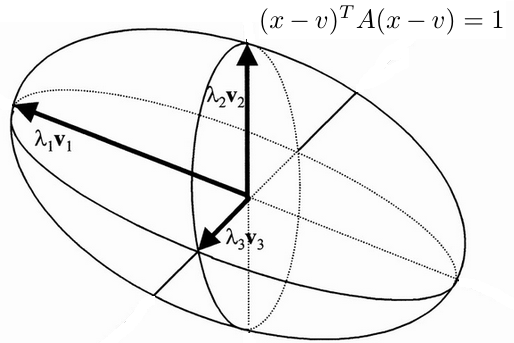
\includegraphics[width=0.5\textwidth]{ellipsoid_eigenvalues.png}
\end{center}

An arbitrarily oriented $n$-dimension ellipsoid $E$, centered at $v$, is defined by the solutions $x$ to the equation $(x-v)^TA(x-v)=1$, where $A$ is a positive definite matrix. What's more, $E$'s axes are in directions of $A$'s eigenvectors, the lengths of axes are $A$'s eigenvalues.


\section{}
Part 1. $A^TA$ is semi-definite

$A^TA$ is symmetric. What's more, it's semi-definite because $x^TA^TAx=(Ax)^TAx=||Ax||^2$.
\\\\ Part 2. Similar matrix

$A$ and $B$ are similar means, for some $M$, $B=M^{-1}AM$. The reason why we care about similar matrix is that they have the same eigenvalues. 

Proof: $Ax=\lambda x \Rightarrow AMM^{-1}x=\lambda x \Rightarrow M^{-1}AMM^{-1}x=\lambda M^{-1}x \Rightarrow BM^{-1}x=\lambda M^{-1}x \Rightarrow Bx'=\lambda x'$.


\section{}
Part 1.Singular-value decomposition(SVD)

For a matrix $A$, we can find an orthonormal basis $v_1, v_2, \cdots, v_n$ for its row space and an orthonormal basis $u_1, u_2, \cdots, u_n$ for its column space. We can get the connection of $u_i$ and $v_i$ with $Av_i=\sigma_i u_i$, or in matrix form, $AV=U\Sigma$. Since $V$ is orthonormal, $A=U \Sigma V^T$, which is called {\bfseries Singular-value decomposition(SVD)}. We can calculate $U, \Sigma, V$ with(proof below): $U$ is the eigenvector matrix of $AA^T$, $V$ is the eigenvector of $A^TA$, $\Sigma$ is the positive sqrt of eigenvalues of both $A^TA$ and $AA^T$. 

Proof: $A=U \Sigma V^T \Rightarrow A^TA=V\Sigma^T U^TU \Sigma V^T=V(\Sigma^T \Sigma) V^T$. Since $A^TA$ is square symmetric, we know $V(\Sigma^T \Sigma) V^T$ is eigen-decomposition of $A^TA$, where the eigenvectors is orthonormal(22.2.a). So we know $V$ and $\Sigma$ exactly. And get $U$ with $AA^T$ in the same way.

The meaning of $A=U \Sigma V^T$ is as below, where $r$ is $A$'s rank: 

$v_1, v_2, \cdots, v_r$ is the orthonormal basis for $A$'s row space;

$u_1, u_2, \cdots, u_r$ is the orthonormal basis for $A$'s column space; 

$v_r, v_{r+1}, \cdots, v_n$ is the orthonormal basis for $A$'s nullspace; 

$u_r, u_{r+1}, \cdots, u_n$ is the orthonormal basis for $A^T$'s nullspace.
\\\\ Part 2. Relation and difference between eigen-decomposition and SVD

Relation: You see that when $U=V$, $A=U \Sigma V^T$ becomes eigen-decomposition that $A=U \Sigma U^T$. This happens when $A^TA=AA^T$ from the proof in part1. Matrix $A$ is called {\bfseries normal matrix} if $A^TA=AA^T$ or $A^HA=AA^H$. So SVD is the generalization of the eigen-decomposition of a positive semi-definite normal matrix. 

Difference: The eigenvalue decomposition and SVD differ except for positive semi-definite normal matrices. For further detail, see SVD on wikipedia, section of \textit{Relation to eigenvalue decomposition}.

\section{}
\hspace*{0.5cm} This section is very simple that the linear transformation can describe phenomenons in real world.

\section{}
\hspace*{0.5cm} Let's compress an image with JPEG! Say, for a 512*512 gray image, first, divide it by 8*8 blocks. Then each block $b$ is a vector with length of 64, originally described by 64 numbers and standard basis $V$ as $b=\sum b_i v_i$. The standard basis is like $[1, 0, 0]^T, [0, 1, 0]^T, [0, 0, 1]^T$ in three dimension space. To compress the image, we change the basis matrix with Fourier matrix $F$ for each block. Then we present each block as $b=\sum c_i f_i$, further more, we only reserve a little(usually 2 or 3) $c_i$s to approximate $b$. 

1. You see that instead 64 numbers, we now only need a little(2 or 3) numbers to store each block, thus also to the whole image. 

2.  You can also see that the standard basis is not good to reserve only a little $c_i$s in $b=\sum c_i f_i$. That's why we change the basis.

3. Wavelet basis is also used in JPEG-2000, the simplest wavelet basis is like:
\begin{center}
	$
	\begin{bmatrix} 1 \\ 1 \\ 1 \\ 1 \\ 1 \\ 1 \\ 1 \\ 1 \end{bmatrix},
	\begin{bmatrix} 1 \\ 1 \\ 1 \\ 1 \\ -1 \\ -1 \\ -1 \\ -1 \end{bmatrix},		\begin{bmatrix} 1 \\ 1 \\ -1 \\ -1 \\ 0 \\ 0 \\ 0 \\ 0 \end{bmatrix},
	\begin{bmatrix} 0 \\ 0 \\ 0 \\ 0 \\1 \\ 1 \\ -1 \\ -1 \end{bmatrix},
	\begin{bmatrix} 1 \\ -1 \\ 0 \\ 0 \\ 0 \\ 0 \\ 0 \\ 0 \end{bmatrix},
	\begin{bmatrix} 0 \\ 0 \\ 1 \\ -1 \\ 0 \\ 0 \\ 0 \\ 0 \end{bmatrix},
	\begin{bmatrix} 0 \\ 0 \\ 0 \\ 0 \\ 1 \\ -1 \\ 0 \\ 0 \end{bmatrix},
	\begin{bmatrix} 0 \\ 0 \\ 0 \\ 0 \\ 0 \\ 0 \\ 1 \\ -1 \end{bmatrix},
	$
\end{center}

4. Apparently, we want a good basis $P$ to do both decompression $b=Pc$ and compression $c=P^{-1}b$ fast. So you see the wavelet basis in 3 of course is fast in computer, since it only contains $1$ and $-1$. 

The algorithms to change basis with Fourier basis or wavelet basis is called {\bfseries Fast Fourier transform(FFT), Fast wavelet transform(FWT)}. 

5. From 3 and 4, you see that basis is very important. Because basis the path we analyze our data/signal, for example, we can change the basis along time with along frequency, which is core idea of FFT and FWT that makes things easily.

\section{}
\hspace*{0.5cm} Quiz review.

\section{}

\end{spacing}
\end{document}